\section{Проектирование системы мониторинга рисков и обеспечения безопасности путешественников}
\label{sec:designing}

В данном разделе приведено описание функциональных требований, архитектурное проектирование компонентов системы и детальное описание структуры данных и алгоритмов взаимодействия. Проектирование выполнено с учетом выявленных в ходе анализа требований к масштабируемости, отказоустойчивости и скорости обработки данных.

\subsection{Функциональные требования и сценарии использования}

Система ориентирована на две основные группы пользователей: путешественники (конечные пользователи) и администраторы системы (для мониторинга состояния сервисов и управления инфраструктурой).

Основные сценарии использования включают:
\begin{itemize}
    \item \textbf{регистрация и настройка профиля:} пользователь указывает свои предпочтения по типам уведомлений (например, только террористические акты и природные катастрофы) и задает критические уровни опасности, при которых система должна прерывать текущий маршрут;
    \item \textbf{просмотр глобальной интерактивной карты рисков:} визуализация актуальных событий в реальном времени, пользователь может видеть точки инцидентов, зоны их влияния (полигоны) и фильтровать их по категориям, дате и уровню значимости.
    \item \textbf{интеллектуальный мониторинг маршрута:} при вводе планируемого маршрута система автоматически проводит пространственный анализ на пересечение пути с зонами активных инцидентов, в случае обнаружения опасности система предлагает альтернативные варианты или выводит предупреждение;
    \item \textbf{автоматическое получение уведомлений:} рассылка push-сообщений при вхождении пользователя в зону риска (геофенсинг) или при возникновении нового критического события в радиусе 50-100 км от текущего местоположения туриста;
    \item \textbf{администрирование и мониторинг:} системный администратор имеет возможность отслеживать статус работы всех микросервисов, скорость обработки очередей в RabbitMQ и корректность загрузки данных из проекта GDELT.
\end{itemize}

\begin{figure}[h]
    \centering
    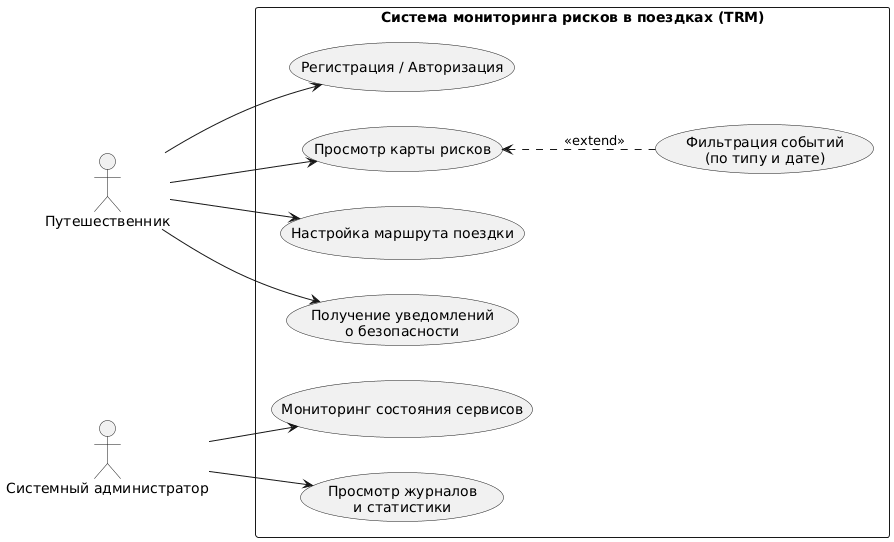
\includegraphics[width=1\textwidth]{picture/diagramm/use_case_diagramm.png}
    \caption{Диаграмма вариантов использования (Use Case Diagram)}
    \label{fig:use_case_diagram}
\end{figure}

\subsection{Архитектура системы}

Для реализации требований к высокой доступности и возможности независимого обновления компонентов выбрана микросервисная архитектура. На рисунке \ref{fig:component_diagram} представлена общая схема взаимодействия компонентов.

\begin{figure}[h]
    \centering
    
\includegraphics[width=1.0\textwidth]{picture/diagramm/components_diagramm.png}
    \caption{Диаграмма компонентов системы}
    \label{fig:component_diagram}
\end{figure}

Система состоит из трех ключевых функциональных модулей:

\subsubsection{Модуль сбора данных}

Данный микросервис реализован на языке Python и отвечает за непрерывный сбор первичной информации из внешних источников.
\begin{itemize}
    \item \textbf{цикл обновления:} согласно регламенту GDELT, новые данные публикуются каждые 15 минут, этот модуль работает по таймеру, инициируя загрузку архивов;
    \item \textbf{обработка форматов:} сервис скачивает сжатые CSV-файлы (события, упоминания и граф знаний), распаковывает их и преобразует в структурированные записи;
    \item \textbf{изоляция данных:} для предотвращения потери информации все сырые данные сохраняются в промежуточной базе данных, что позволяет, при необходимости, повторно запустить процесс анализа с новыми алгоритмами;
    \item \textbf{межсервисная связь:} после завершения загрузки порции данных в RabbitMQ отправляется событие, содержащее список идентификаторов для последующего анализа.
\end{itemize}

\subsubsection{Модуль интеллектуального анализа событий}

Это вычислительное ядро системы, использующее современные модели машинного обучения для извлечения смысла из текстовых данных. Алгоритм работы модуля представлен на рисунке \ref{fig:analyzer_flow}.

\begin{figure}[h]
    \centering
    
\includegraphics[width=1.0\textwidth]{picture/diagramm/analyzer_flow.png}
    \caption{Алгоритм обработки события в модуле Analyzer}
    \label{fig:analyzer_flow}
\end{figure}

Ключевые этапы анализа:
\begin{itemize}
    \item \textbf{скрапинг и очистка:} по ссылке из GDELT извлекается полный текст статьи, применяются алгоритмы удаления рекламы, скриптов и навигационных элементов;
    \item \textbf{семантическая классификация:} использование модели DeBERTa-v3 для Zero-shot классификации, что это позволяет сопоставлять новость с типами угроз (например, «Авиакатастрофа», «Забастовка аэропорта») без жесткой привязки к ключевым словам;
    \item \textbf{продвинутый геопарсинг:} извлечение точных координат упоминаемых мест с помощью Mordecai 3, то есть, если в тексте упоминается несколько локаций, система строит выпуклую оболочку для определения зоны влияния события;
    \item \textbf{реферирование и генерация:} использование локальной LLM Qwen2.5 (через Ollama) для создания краткой сводки,  это критически важно для отправки лаконичных уведомлений на мобильные устройства.
\end{itemize}

\subsubsection{Серверная часть приложения}

Микросервис на Java, управляющий состоянием системы и пользовательскими данными.
\begin{itemize}
    \item \textbf{управление пространственными данными:} использование Hibernate Spatial для работы с геометрическими типами данных PostGIS;
    \item \textbf{логика геофенсинга:} при сохранении нового события система выполняет запрос к базе данных для поиска пересечений зоны риска с текущими местоположениями активных пользователей;
    \item \textbf{API Gateway:} предоставление единой точки входа для клиентских приложений с авторизацией на основе JWT-токенов.
\end{itemize}

\subsection{Взаимодействие компонентов системы}

На рисунке \ref{fig:seq_main_flow} приведена диаграмма последовательности, иллюстрирующая жизненный цикл обработки события — от его публикации в GDELT до появления уведомления на устройстве пользователя.

\begin{figure}[h]
    \centering
    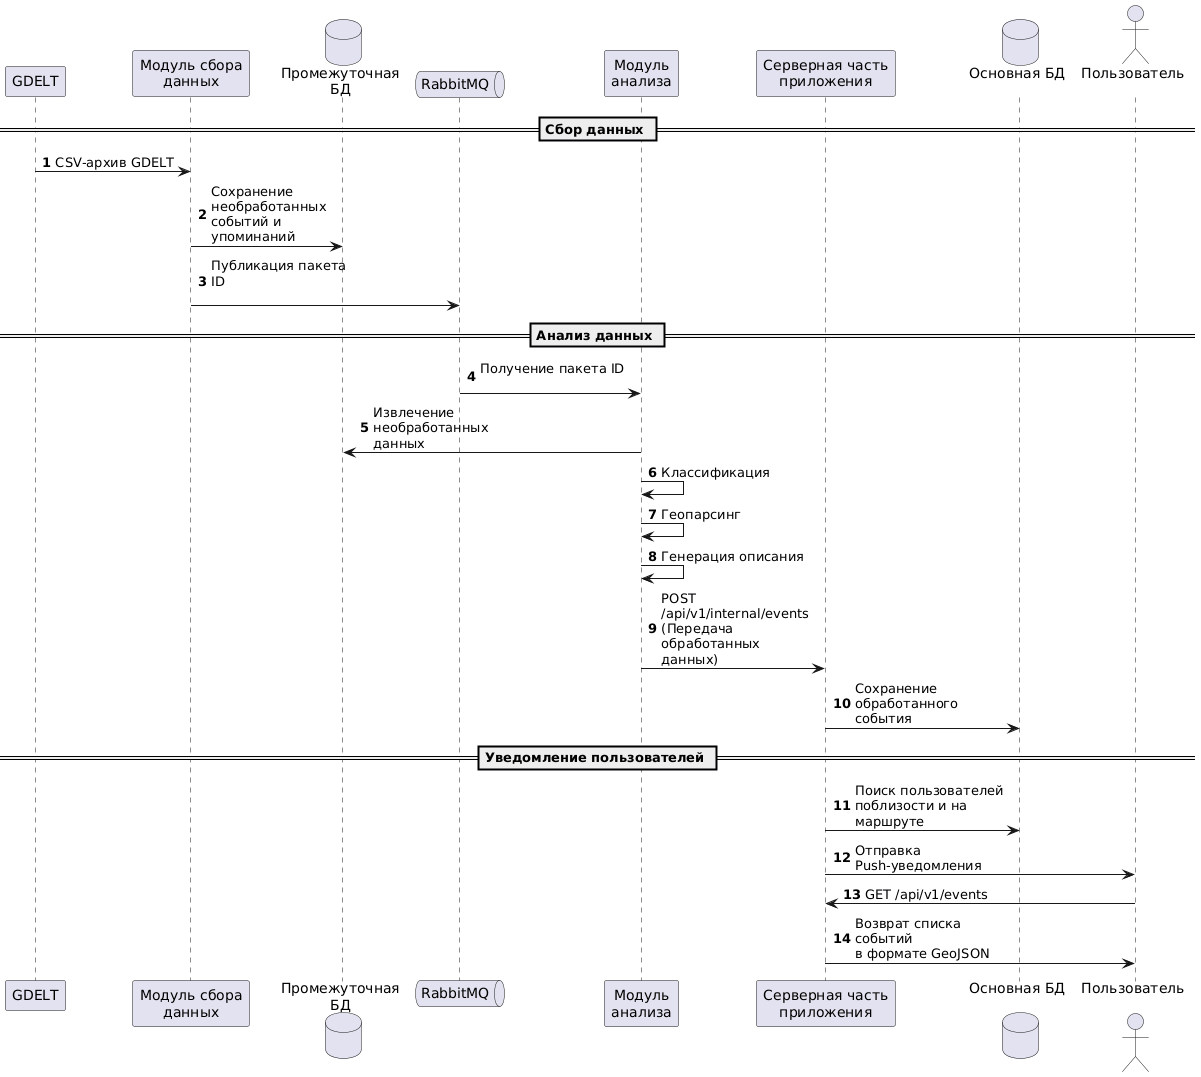
\includegraphics[width=1\textwidth]{picture/diagramm/seq_diagramm.png}
    \caption{Диаграмма последовательности обработки события}
    \label{fig:seq_main_flow}
\end{figure}

Процесс включает следующие шаги:
\begin{itemize}
    \item загрузка CSV-архива и сохранение в промежуточную базу данных;
    \item публикация сообщения в очередб сообщений;
    \item асинхронный захват задачи модулем Analyzer;
    \item выполнение NLP-конвейера (классификация, геопарсинг, LLM-реферирование);
    \item передача структурированного объекта в серверную часть приложения;
    \item поиск затронутых пользователей и отправка Push-уведомления через Firebase Cloud Messaging.
\end{itemize}

\subsection{Проектирование структуры базы данных}

База данных спроектирована с разделением на промежуточное и основное хранилище для обеспечения чистоты данных и возможности масштабирования аналитики. Схема классов и связей представлена на рисунке \ref{fig:db_schema_main}.

\begin{figure}[h]
    \centering
    
\includegraphics[width=1\textwidth]{picture/diagramm/class_diagramm.png}
    \caption{Схема классов и связей в базе данных (Class Diagram)}
    \label{fig:db_schema_main}
\end{figure}

\subsubsection{Промежуточное хранилище}

Таблицы в данном контуре максимально приближены к формату GDELT:
\begin{itemize}
    \item \textbf{gdelt\_events:} хранит базовую информацию о событиях (тип действия, страна, первичные координаты);
    \item \textbf{gdelt\_mentions:} содержит ссылки на все источники, упоминающие данное событие;
    \item \textbf{raw\_articles:} кэширует извлеченный текст статей для снижения нагрузки на внешние новостные ресурсы.
\end{itemize}

\subsubsection{Основное хранилище}

Оптимизировано для работы ГИС-функций и мобильного приложения:
\begin{itemize}
    \item \textbf{events:} очищенные события с геометрией (тип Geometry), уровнем критичности и мультиязычным описанием;
    \item \textbf{users:} данные профиля, настройки приватности и предпочтения фильтрации;
    \item \textbf{routes:} планируемые маршруты пользователей в виде линейных геометрий (LineString);
    \item \textbf{audit Log:} история срабатывания уведомлений и действий администратора.
\end{itemize}

\subsection{Проектирование программных интерфейсов}

Для взаимодействия фронтенда и бэкенда используется RESTful API, соответствующий спецификации OpenAPI 3.0.

Основные эндпоинты системы:
\begin{itemize}
    \item \textbf{GET /api/v1/events/map:} возвращает массив событий в формате GeoJSON для отображения на карте MapLibre, поддерживает параметры фильтрации по bounding box (bbox);
    \item \textbf{POST /api/v1/user/location:} регулярное обновление координат пользователя для работы алгоритма геофенсинга;
    \item \textbf{POST /api/v1/trips/analyze:} отправка планируемого маршрута для получения отчета о безопасности, возвращает список точек пересечения с зонами риска;
    \item \textbf{GET /api/v1/notifications/history:} получение истории уведомлений для конкретного пользователя.
\end{itemize}

Для обеспечения высокой скорости работы аналитического конвейера взаимодействие между анализатором и сервыерной частью приложения может осуществляться через протокол gRPC, что снижает накладные расходы на сериализацию данных по сравнению со стандартным REST.
